\section{Road Map}

\begin{figure}[t]
\centering
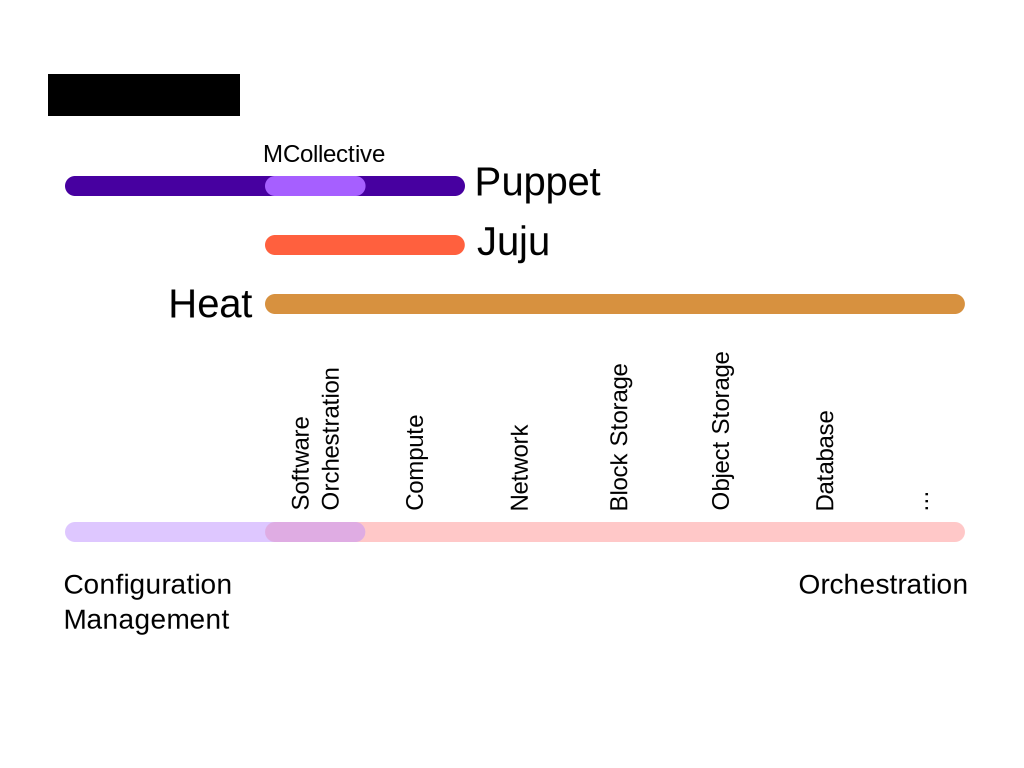
\includegraphics[trim=0em 8em 0em 15em,width=\textwidth]{orchestration-config-management.pdf}
\caption{The relative positioning of Heat compared with other categories of software: configuration management systems (such as Puppet or Chef) and configuration managment--orchestration hybrids (such as Juju).}
\label{fig:orchestration-config-management}
\end{figure}

The \textsc{Hot} format is an effort to develop a native template language for Heat.\footnote{Note that support for the CloudFormation template format will be maintained indefinitely.} Most of the changes prototyped so far are only cosmetic in nature, and are aimed at taking advantage of a \textsc{Yaml}-native format to improve readability of templates.

However, the long-term plan is to enhance \textsc{Hot} to the point where it can handle the same sorts of complex application topologies as \textsc{Tosca}. The main way to do this is to allow orchestration between software components in a similar way as we do with infrastructure components.

In proposals currently under discussion, this would be implemented using software configurations that are not tied to a particular server. Multiple configurations could be hosted on the same server, or split up to different servers depending on the environment. (For example, you could define Database and Application configurations an co-locate them on a single server for testing but separate them for production.)

As with infrastructure, dependencies would be inferred from configuration data relationships between resources in the template. Heat would handle instantiating software services with the correct timing, and passing data between them.
